\documentclass[aspectratio=169, 10pt]{beamer}

% ============================================================
% Lecture 1: 'Cause We Are Living in a Counterfactual World
% Counterfactual Framework and Selection-on-Observables
% PhD programme: Economics, Management and Methods for the
% Sustainable Transition — University of Ferrara, 5 May 2026
% Author: Francesco Rentocchini
% ============================================================

\usetheme{default}
% ============================================================
% preamble.tex — fit_phd_lectures
% Adapted from Scott Cunningham's Causal Inference Mixtape Sessions
% Compatible with pdflatex
% ============================================================

% --- Colors — JRC / European Commission identity ------------
\usepackage{xcolor}

% EC / JRC brand palette — softer pastel-leaning blue
\definecolor{ecblue}{HTML}{2E75B6}    % JRC pastel blue (softer than flag blue)
\definecolor{jrcblue}{HTML}{5B9BD5}   % JRC lighter accent blue
\definecolor{eugold}{HTML}{FFCC00}    % EU flag gold
\definecolor{ecnavy}{HTML}{1F3864}    % deep navy for text / headers
\definecolor{ecgray}{HTML}{54585A}    % EC institutional gray
\definecolor{ecred}{HTML}{C0392B}     % alert / warning red
\definecolor{ecgreen}{HTML}{1E7D34}   % example / positive green
\definecolor{lightblue}{HTML}{DEEBF7} % light blue tint for block bodies
\definecolor{offwhite}{HTML}{F7F8FC}  % near-white slide bg

% Convenience aliases
\definecolor{accent}{HTML}{2E75B6}    % = ecblue
\definecolor{accent2}{HTML}{C0392B}   % = ecred
\definecolor{gray100}{HTML}{DEEBF7}   % = lightblue
\definecolor{gray800}{HTML}{1F3864}   % = ecnavy

% Legacy aliases (used in slide source — map to JRC equivalents)
\definecolor{jet}{HTML}{1B2A6B}       % was near-black, now ecnavy
\definecolor{asher}{HTML}{54585A}     % was mid-gray, now ecgray
\definecolor{daisy}{HTML}{FFCC00}     % was yellow, now eugold
\definecolor{alice}{HTML}{0065A2}     % was teal, now jrcblue
\definecolor{coral}{HTML}{C0392B}     % was orange-red, now ecred
\definecolor{ruby}{HTML}{C0392B}      % was dark red, now ecred
\definecolor{kelly}{HTML}{1E7D34}     % was olive, now ecgreen
\definecolor{cranberry}{HTML}{C0392B} % was pink-red, now ecred

% --- Beamer theme — JRC style -------------------------------
\setbeamercolor{background canvas}{bg = white}
\setbeamersize{text margin left = 15pt, text margin right = 15pt}

% Frame title: white text on EC blue bar
\setbeamercolor{frametitle}{bg = ecblue, fg = white}
\setbeamercolor{framesubtitle}{bg = ecblue, fg = eugold}
\setbeamerfont{frametitle}{size = \normalsize, series = \bfseries}
\setbeamerfont{framesubtitle}{size = \small, shape = \itshape}

% Alerts
\setbeamercolor{alerted text}{fg = ecred}

% Blocks
\setbeamercolor{block title}{fg = white, bg = ecblue}
\setbeamercolor{block body}{fg = ecnavy, bg = lightblue}
\setbeamercolor{alertblock title}{fg = white, bg = ecred}
\setbeamercolor{alertblock body}{fg = ecnavy, bg = lightblue}
\setbeamercolor{exampleblock title}{fg = ecnavy, bg = eugold}
\setbeamercolor{exampleblock body}{fg = ecnavy, bg = lightblue}

% Title page — clean JRC style: white bg, left blue stripe, dark title text
% Slide canvas: 160mm × 90mm (aspectratio=169)
\setbeamercolor{title}{fg = ecnavy}
\setbeamercolor{subtitle}{fg = ecblue}
\setbeamerfont{title}{size = \LARGE, series = \bfseries}
\setbeamertemplate{title page}{%
    \begin{tikzpicture}[remember picture, overlay]
        % Left blue stripe (12mm wide, full height)
        \fill[ecblue] (current page.north west)
            rectangle ([xshift=12mm]current page.south west);
        % Gold horizontal accent line (~60% width, vertically centred below title)
        \draw[eugold, line width=2.5pt]
            ([xshift=16mm, yshift=-43mm]current page.north west) --
            ([xshift=150mm, yshift=-43mm]current page.north west);
        % Title — large, dark navy, on white area
        \node[anchor=north west, text width=136mm, align=left,
              font=\LARGE\bfseries, text=ecnavy]
            at ([xshift=16mm, yshift=-9mm]current page.north west)
            {\inserttitle};
        % Subtitle — below gold line, in pastel blue italic
        \node[anchor=north west, text width=136mm, align=left,
              font=\normalsize\itshape, text=ecblue]
            at ([xshift=16mm, yshift=-49mm]current page.north west)
            {\insertsubtitle};
        % Author — bold navy
        \node[anchor=north west, text width=136mm, align=left,
              font=\normalsize\bfseries, text=ecnavy]
            at ([xshift=16mm, yshift=-66mm]current page.north west)
            {\insertauthor};
        % Institution · date — small gray
        \node[anchor=north west, text width=136mm, align=left,
              font=\small, text=ecgray]
            at ([xshift=16mm, yshift=-74mm]current page.north west)
            {\insertinstitute\ \textbullet\ \insertdate};
    \end{tikzpicture}%
}

% TOC
\setbeamercolor{section in toc}{fg = ecblue}
\setbeamercolor{subsection in toc}{fg = ecnavy}

% Navigation
\setbeamertemplate{navigation symbols}{}

% Footer: thin gold line + institution name left, slide number right
\setbeamertemplate{footline}{%
    \begin{beamercolorbox}[wd=\paperwidth, ht=0.4pt]{frametitle}%
        \color{eugold}\rule{\paperwidth}{0.4pt}%
    \end{beamercolorbox}%
    \begin{beamercolorbox}[wd=\paperwidth, ht=5pt, dp=3pt,
            leftskip=6pt, rightskip=6pt]{normal text}%
        {\color{ecgray}\tiny F. Rentocchini / European Commission, JRC-Seville \& DEMM, University of Milan \hfill
         \color{ecgray}\tiny \ifnum\insertframenumber>1 \insertframenumber\fi}%
    \end{beamercolorbox}%
}

% Bullet points
\settowidth{\leftmargini}{\usebeamertemplate{itemize item}}
\addtolength{\leftmargini}{\labelsep}
\setbeamercolor{enumerate item}{fg = ecblue}
\setbeamertemplate{enumerate item}{\insertenumlabel.}
\setbeamercolor{itemize item}{fg = ecblue}
\setbeamertemplate{itemize item}[circle]
\setbeamercolor{itemize subitem}{fg = jrcblue}
\setbeamertemplate{itemize subitem}{$\rightarrow$}

% --- Section transition frames — EC blue bg, gold text ------
\newenvironment{transitionframe}{
    \setbeamercolor{background canvas}{bg = ecblue}
    \begin{frame}\color{white}\LARGE\centering
}{
    \end{frame}
}

% --- Auto-roadmap at each section ---------------------------
\AtBeginSection[]{
    \begin{frame}{Roadmap}
        \tableofcontents[currentsection]
    \end{frame}
}

% --- Packages -----------------------------------------------
\usepackage{amsmath, amssymb, amsthm}
\usepackage{graphicx}
\usepackage{booktabs}
\usepackage{array, adjustbox, tabularx}
\usepackage{threeparttable}
\usepackage{setspace}
\setstretch{1.15}
\usepackage{multicol}
\usepackage[protrusion=false,expansion=false]{microtype}
\usepackage{hyperref}
\hypersetup{colorlinks=true, linkcolor=accent2, urlcolor=accent2, citecolor=accent2}
\pdfstringdefDisableCommands{%
  \def\translate#1{#1}%
  \def\color#1{}%
}

% --- TikZ for DAGs ------------------------------------------
\usepackage{tikz}
\usetikzlibrary{positioning, arrows.meta, shapes.geometric, calc, fit}

% DAG style shortcuts
\tikzset{
    node/.style = {circle, draw=accent, fill=gray100, thick,
                   minimum size=8mm, font=\small},
    latent/.style = {circle, draw=accent, dashed, fill=white, thick,
                     minimum size=8mm, font=\small},
    arrow/.style = {-{Stealth[length=6pt]}, thick, color=jet},
    redarrow/.style = {-{Stealth[length=6pt]}, thick, color=accent2},
    bluearrow/.style = {-{Stealth[length=6pt]}, thick, color=accent},
}

% --- Highlighting box for equations -------------------------
\newcommand{\highlight}[1]{%
    \colorbox{eugold!50}{$\displaystyle #1$}}

% --- Fix \input with tables ---------------------------------
\makeatletter
\let\input\@@input
\makeatother

% Suppress overfull warnings
\vfuzz2pt
\hfuzz2pt


\usepackage{natbib}
\bibliographystyle{apalike}

% --- Title ---------------------------------------------------
\title['Cause We Are Living in a Counterfactual World]{%
  `Cause We Are Living in a Counterfactual World}
\subtitle{Counterfactual Framework and Selection on Observables\\
  \small Lecture 1 --- PhD Economics, Management and Methods for the Sustainable Transition,University of Ferrara}
\author{Francesco Rentocchini}
\institute{JRC European Commission / University of Milan}
\date{5 May 2026}

% ============================================================
\begin{document}
% ============================================================

\begin{frame}
  \titlepage
\end{frame}

\begin{frame}{Today's roadmap}
  \tableofcontents
\end{frame}

% ============================================================
\section{Motivation: Why Causality?}
% ============================================================

\begin{frame}{Correlation is not causation — and it matters}

  \begin{columns}[T]
    \begin{column}{0.55\textwidth}
      \begin{itemize}
        \item Countries with more storks have higher birth rates
        \item Ice-cream sales predict drowning deaths
        \item Hospitals kill more people than battlefields
      \end{itemize}
      \bigskip
      All three statements are \alert{true correlations} and \alert{useless}.

      \bigskip
      \begin{block}{The policy question}
        Does \emph{this programme} improve outcomes for the people who receive it?
        What would have happened to them \emph{without} it?
      \end{block}
    \end{column}
    \begin{column}{0.4\textwidth}
      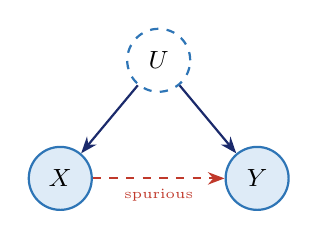
\begin{tikzpicture}
        \node[node] (X) at (0,0) {$X$};
        \node[node] (Y) at (2.5,0) {$Y$};
        \node[latent] (U) at (1.25, 1.5) {$U$};
        \draw[arrow] (U) -- (X);
        \draw[arrow] (U) -- (Y);
        \draw[redarrow, dashed] (X) -- node[below,font=\tiny,color=accent2]{spurious} (Y);
      \end{tikzpicture} \\
      \vspace{2mm}
      \small A common cause $U$ creates a correlation between $X$ and $Y$ even when $X$ has \emph{no} causal effect on $Y$.
    \end{column}
  \end{columns}
\end{frame}

% ------------------------------------------------------------

\begin{frame}{The ventilator problem}

  \begin{columns}[T]
    \begin{column}{0.55\textwidth}
      \begin{itemize}
        \item ICU observation: ventilated patients die \emph{more} often
        \item Naive conclusion: \alert{ventilators kill?} — obviously wrong
        \item Why? Ventilated patients were \textbf{already sicker}
        \item They were selected into treatment \emph{because} of severity
      \end{itemize}

      \medskip
      \begin{block}{The fundamental question}
        What would have happened to ventilated patients\\
        had they \emph{not} been ventilated?\\[3pt]
        That is the \alert{counterfactual} — unobservable by definition.\\
        \emph{Causal inference is the science of disciplined guessing.}
      \end{block}
    \end{column}
    \begin{column}{0.4\textwidth}
      \begin{tabular}{lcc}
        \toprule
        Patient & Ventilated & Survived \\
        \midrule
        Alice   & Yes & No  \\
        Bob     & Yes & No  \\
        Carol   & No  & Yes \\
        Dan     & No  & Yes \\
        \midrule
        \multicolumn{2}{l}{Naive $\Delta$ survival} & \alert{$-$ve} \\
        \bottomrule
      \end{tabular} \\
      \vspace{4mm}
      \small Alice and Carol are not comparable: \textbf{selection into treatment is not random}.
    \end{column}
  \end{columns}
\end{frame}

% ------------------------------------------------------------

\begin{frame}{Three roads to a causal answer}

  \begin{block}{Today: Selection on observables}
    We assume all confounders are \emph{measured}. Estimators: matching, IPW, doubly robust.
  \end{block}

  \begin{exampleblock}{Lecture 2: Quasi-experiments — DiD}
    We exploit \emph{variation in timing} of a policy to construct a counterfactual trend.
  \end{exampleblock}

  \begin{alertblock}{Lecture 3: Quasi-experiments — RDD and Shift-Share IV}
    We exploit \emph{discontinuities} or \emph{external shocks} to extract exogenous variation.
  \end{alertblock}

  \bigskip
  \centering
  All three methods answer the same question with different \textbf{identifying assumptions}. \\
  The assumption is always a claim about the data-generating process — not about the data itself.
\end{frame}

% ============================================================
\section{The Potential Outcomes Framework}
% ============================================================

\begin{frame}{Rubin's potential outcomes notation}

  Let $i = 1, \ldots, N$ index units (firms, individuals, countries).

  \bigskip
  \begin{tabular}{ll}
    $D_i \in \{0,1\}$ & Treatment indicator ($1$ = treated, $0$ = control) \\[4pt]
    $Y_i(1)$ & Outcome unit $i$ \emph{would} realise \textbf{if treated} \\[4pt]
    $Y_i(0)$ & Outcome unit $i$ \emph{would} realise \textbf{if not treated} \\[4pt]
    $\delta_i = Y_i(1) - Y_i(0)$ & \textbf{Individual treatment effect} \\
  \end{tabular}

  \bigskip
  \textbf{Switching equation} — what we actually observe:
  \[
    Y_i = D_i \cdot Y_i(1) + (1 - D_i) \cdot Y_i(0)
  \]

  \bigskip
  \begin{alertblock}{Key insight}
    $Y_i(1)$ and $Y_i(0)$ both exist in principle for every unit.
    We observe at most \emph{one} of them. The other is the \textbf{counterfactual}.
  \end{alertblock}
\end{frame}

% ------------------------------------------------------------

\begin{frame}{The fundamental problem of causal inference}

  \begin{columns}[T]
    \begin{column}{0.5\textwidth}
      \begin{tabular}{lccc}
        \toprule
        Unit & $D_i$ & $Y_i(1)$ & $Y_i(0)$ \\
        \midrule
        Alice  & 1 & 1 & \alert{?} \\
        Bob    & 1 & 0 & \alert{?} \\
        Carol  & 0 & \alert{?} & 1 \\
        Dan    & 0 & \alert{?} & 0 \\
        \bottomrule
      \end{tabular}

      \vspace{4mm}
      \small \alert{?} = never observed. This is a \textbf{missing data problem}, always.
    \end{column}
    \begin{column}{0.46\textwidth}
      \textbf{Average treatment effects:}
      \begin{align*}
        \text{ATE} &= E[Y_i(1) - Y_i(0)] \\[4pt]
        \text{ATT} &= E[Y_i(1) - Y_i(0) \mid D_i = 1] \\[4pt]
        \text{ATU} &= E[Y_i(1) - Y_i(0) \mid D_i = 0]
      \end{align*}

      \vspace{2mm}
      \begin{block}{Which parameter?}
        \textbf{ATT} = effect on those who \emph{chose} to be treated. Most policy-relevant when treatment is voluntary.\\[2pt]
        \textbf{ATE} = effect if we assigned treatment \emph{randomly} to the population.
      \end{block}
    \end{column}
  \end{columns}
\end{frame}

% ------------------------------------------------------------

\begin{frame}{Selection bias: what goes wrong with naive comparisons}

  \textbf{Step 1.} The naive estimator compares treated to untreated:
  \[
    \underbrace{E[Y_i \mid D_i=1] - E[Y_i \mid D_i=0]}_{\text{Simple Difference in Outcomes (SDO)}}
  \]

  \begin{overprint}

  \onslide<1>
    \medskip
    \begin{block}{What does SDO actually measure?}
      We observe $Y_i = D_i Y_i(1) + (1-D_i)Y_i(0)$, so:
      \[
        E[Y_i\mid D_i=1] = E[Y_i(1)\mid D_i=1], \quad
        E[Y_i\mid D_i=0] = E[Y_i(0)\mid D_i=0]
      \]
      SDO mixes the treatment effect \emph{and} pre-existing differences.
    \end{block}

  \onslide<2>
    \medskip
    \textbf{Step 2.} Add and subtract $E[Y_i(0)\mid D_i=1]$:
    \begin{align*}
      \text{SDO}
        &= E[Y_i(1)\mid D_i=1] - E[Y_i(0)\mid D_i=0] \\
        &= E[Y_i(1)\mid D_i=1] \;{\color{ecblue}-\; E[Y_i(0)\mid D_i=1]}
           \;{\color{ecblue}+\; E[Y_i(0)\mid D_i=1]} - E[Y_i(0)\mid D_i=0]
    \end{align*}
    \small (Add and subtract the \emph{unobserved} baseline of the treated group.)

  \onslide<3>
    \medskip
    \textbf{Step 3.} Rearrange — two terms emerge:
    \begin{align*}
      \text{SDO}
        &= \underbrace{E[Y_i(1) - Y_i(0)\mid D_i=1]}_{\text{ATT}}
           + \underbrace{E[Y_i(0)\mid D_i=1] - E[Y_i(0)\mid D_i=0]}_{\alert{\text{Selection bias}}}
    \end{align*}
    \small Selection bias $=$ difference in \emph{untreated} potential outcomes between the two groups.

  \onslide<4->
    \medskip
    \textbf{Step 4.} With heterogeneous effects, SDO also picks up a third term:
    \begin{align*}
      \text{SDO}
        &= \underbrace{E[Y_i(1) - Y_i(0)\mid D_i=1]}_{\text{ATT}}
           + \underbrace{E[Y_i(0)\mid D_i=1] - E[Y_i(0)\mid D_i=0]}_{\alert{\text{Selection bias}}} \\
        &\quad + (1-\pi)\underbrace{(\text{ATT} - \text{ATU})}_{\text{Heterogeneity bias}}
    \end{align*}
    \smallskip
    \begin{itemize}
      \item SDO $=$ ATT \emph{only if} selection bias $= 0$ (treatment independent of $Y_i(0)$)
      \item Intuition: sicker patients → hospital; harder workers → training; larger firms → M\&A
    \end{itemize}

  \end{overprint}
\end{frame}

% ------------------------------------------------------------

\begin{frame}{SUTVA: the hidden assumption}

  All the above rests on the \textbf{Stable Unit Treatment Value Assumption} (Rubin 1980):

  \bigskip
  \begin{enumerate}
    \item \textbf{No interference:} $Y_i(d)$ does not depend on what treatment $D_j$ unit $j \neq i$ receives
      \begin{itemize}
        \item Violated when: spillovers, general equilibrium effects, peer effects
        \item Example: vaccinating my neighbour affects my infection risk
      \end{itemize}
    \bigskip
    \item \textbf{No hidden treatment variation:} there is only one version of each treatment level
      \begin{itemize}
        \item Violated when: treatment is heterogeneous in practice (e.g., ``training'' differs across providers)
      \end{itemize}
  \end{enumerate}

  \bigskip
  \begin{alertblock}{Keep in mind}
    SUTVA is an assumption about the world, not the data. If it fails, $Y_i(d)$ is not well-defined and the whole framework breaks down. Always ask: could my treated units affect my controls?
  \end{alertblock}
\end{frame}

% ============================================================
\section{Identification: from Description to Causality}
% ============================================================

% ------------------------------------------------------------

\begin{frame}{A first attempt: just add controls to OLS}

  \textbf{Idea:} if the bias comes from omitted variables, why not include them?
  \[
    Y_i = \alpha + \beta D_i + \gamma' X_i + \varepsilon_i
  \]
  $\hat\beta$ identifies ATT \emph{only if} $E[\varepsilon_i \mid D_i, X_i] = 0$ — i.e., no residual confounding.

  \medskip
  \textbf{Read the controls as a diagnostic:}

  \begin{overprint}

  \onslide<1>
    \begin{block}{Coefficient falls after adding controls}
      $\hat\beta^{\text{naive}} > \hat\beta^{\text{OLS+X}}$ — positive selection\\[3pt]
      Treated units had \emph{better} baseline outcomes: e.g.\ more able workers self-select into training.\\
      Controls absorb some of the spurious advantage. \textbf{Good sign} — you are correcting in the right direction.
    \end{block}

  \onslide<2>
    \begin{block}{Coefficient rises after adding controls}
      $\hat\beta^{\text{naive}} < \hat\beta^{\text{OLS+X}}$ — negative selection\\[3pt]
      Treated units had \emph{worse} baseline outcomes: e.g.\ sicker patients received the drug.\\
      The naive estimate was attenuated downward. Controls reveal a larger true effect.
    \end{block}

  \onslide<3>
    \begin{alertblock}{Standard error rises after adding controls}
      Happens when $X$ is \emph{highly collinear} with $D$ — controls absorb most variation in treatment.\\[3pt]
      Extreme case: $X$ is a near-perfect predictor of $D$ $\Rightarrow$ \textbf{multicollinearity}, very imprecise $\hat\beta$.\\
      Also: small within-cell sample sizes inflate SEs even without collinearity.
    \end{alertblock}

  \onslide<4>
    \begin{alertblock}{Standard error falls after adding controls}
      $X$ explains residual variation in $Y$ without being collinear with $D$.\\[3pt]
      Controls reduce $\hat\sigma^2_\varepsilon$ $\Rightarrow$ smaller SEs — more precise estimate.
      This is the \emph{best case}: controls both correct bias \emph{and} improve precision.
    \end{alertblock}

  \onslide<5->
    \begin{alertblock}{Sign flip after adding controls — the most alarming case}
      $\hat\beta^{\text{naive}} > 0$ but $\hat\beta^{\text{OLS+X}} < 0$ (or vice versa).
      Omitted variable was so strongly correlated with $D$ that it \emph{reversed} the raw association.\\[2pt]
      \textbf{Classic examples:} hospitals $\uparrow$ mortality (naive) $\to$ negative after controlling for baseline health; elite schools $\uparrow$ wages (naive) $\to$ near-zero after controlling for ability.\\[2pt]
      \alert{A sign flip is a red flag: OLS with controls may still be insufficient — CIA may not hold.}
    \end{alertblock}

  \end{overprint}
\end{frame}

% ------------------------------------------------------------

\begin{frame}{Random assignment solves the problem}

  If treatment is assigned \textbf{randomly}:
  \[
    D_i \perp \bigl(Y_i(0),\, Y_i(1)\bigr)
  \]
  Then:
  \[
    E[Y_i(0)\mid D_i=1] = E[Y_i(0)\mid D_i=0]
  \]
  Selection bias $= 0$, and SDO $=$ ATE $=$ ATT.

  \bigskip
  \begin{columns}[T]
    \begin{column}{0.48\textwidth}
      \begin{exampleblock}{RCT: the gold standard}
        Random assignment makes the two groups identical in expectation on all characteristics — observed \emph{and} unobserved.
      \end{exampleblock}
    \end{column}
    \begin{column}{0.48\textwidth}
      \begin{alertblock}{The problem}
        We often \emph{cannot} randomise:
        firms self-select into acquiring; workers choose training; countries adopt policies for a reason.
        We need an \emph{assumption} to substitute for randomisation.
      \end{alertblock}
    \end{column}
  \end{columns}
\end{frame}

% ------------------------------------------------------------

\begin{frame}{The Conditional Independence Assumption (CIA)}

  \textbf{Idea:} conditional on observed characteristics $X_i$, treatment assignment is \emph{as good as random}.

  \[
    \bigl(Y_i(0),\, Y_i(1)\bigr) \;\perp\; D_i \;\Big|\; X_i
    \qquad \text{(Unconfoundedness / CIA)}
  \]

  \medskip
  \begin{columns}[T]
    \begin{column}{0.44\textwidth}
      \textbf{What $X_i$ must contain:}
      \begin{itemize}
        \item All variables that jointly determine treatment \emph{and} potential outcomes
        \item I.e., all \textbf{confounders} must be measured
        \item Missing a confounder $\Rightarrow$ CIA fails
      \end{itemize}
    \end{column}
    \begin{column}{0.52\textwidth}
      \begin{center}
      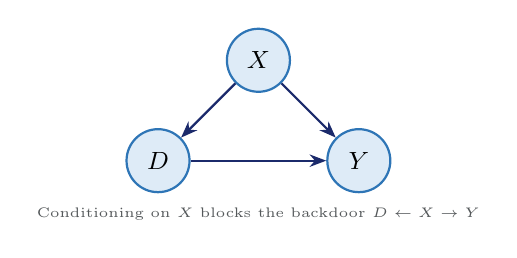
\begin{tikzpicture}[scale=0.85]
        \node[node] (X) at (0,0)   {$X$};
        \node[node] (D) at (-1.5,-1.5) {$D$};
        \node[node] (Y) at (1.5,-1.5)  {$Y$};
        \draw[arrow] (X) -- (D);
        \draw[arrow] (X) -- (Y);
        \draw[arrow] (D) -- (Y);
        \node[font=\tiny, color=asher] at (0,-2.3) {Conditioning on $X$ blocks the backdoor $D\leftarrow X\rightarrow Y$};
      \end{tikzpicture}
      \end{center}
    \end{column}
  \end{columns}

  \bigskip
  \textbf{Common support (overlap):}
  \[
    0 < P(D_i=1 \mid X_i) < 1 \quad \forall\, X_i
  \]
  Every value of $X$ must appear in both treated and control groups. Otherwise, we extrapolate.
\end{frame}

% ============================================================
\section{Estimators for Selection on Observables}
% ============================================================

\begin{frame}{Subclassification}

  \textbf{Idea:} partition the covariate space $X$ into $K$ strata. Within each stratum, CIA holds by construction (units are identical on $X$).

  \[
    \widehat{\tau}^{\text{ATE}} = \sum_{k=1}^{K} \frac{N_k}{N} \cdot \underbrace{\bigl(\bar{Y}_k^{D=1} - \bar{Y}_k^{D=0}\bigr)}_{\text{stratum-specific effect}}
  \]

  \bigskip
  \begin{columns}[T]
    \begin{column}{0.48\textwidth}
      \begin{exampleblock}{Strengths}
        \begin{itemize}
          \item Transparent and interpretable
          \item No functional form imposed
          \item Naturally handles ATE vs.\ ATT (different weights)
        \end{itemize}
      \end{exampleblock}
    \end{column}
    \begin{column}{0.48\textwidth}
      \begin{alertblock}{Weakness}
        \textbf{Curse of dimensionality:} with $p$ binary covariates, you need $2^p$ cells. Many will be empty (no overlap).\\
        \medskip
        \textbf{Solution:} collapse $X$ to a scalar — the \emph{propensity score} — or use coarsened matching.
      \end{alertblock}
    \end{column}
  \end{columns}
\end{frame}

% ------------------------------------------------------------

\begin{frame}{Exact matching and its limits}

  \textbf{Exact matching:} for each treated unit $i$, find a control unit $j$ with identical $X_j = X_i$.

  \[
    \widehat{\delta}_i = Y_i - Y_{j(i)}, \quad
    \widehat{\text{ATT}} = \frac{1}{N_1} \sum_{i: D_i=1} \widehat{\delta}_i
  \]

  \bigskip
  \begin{itemize}
    \item Fully non-parametric: no model for $E[Y|X]$
    \item Estimating is the same as a within-cell comparison
    \item \alert{Breaks down in high dimensions:} with 10 binary covariates, $2^{10} = 1{,}024$ cells; few or none will have both treated and control units
  \end{itemize}

  \bigskip
  \begin{block}{The trade-off}
    Exact matching $\rightarrow$ zero bias, but high variance (few matches, many discarded units).\\
    Inexact / caliper matching $\rightarrow$ lower variance, but introduces bias.
  \end{block}
\end{frame}

% ------------------------------------------------------------

\begin{frame}{Coarsened Exact Matching (CEM)}

  \citet{iacus2012causal}. \textbf{Key idea:} coarsen each covariate into bins, \emph{then} exact-match on the coarsened values.

  \smallskip
  \textbf{Algorithm:}
  \begin{enumerate}
    \item For each $X_k$, define bins (e.g., age: 18–25, 26–35, 36–50, 51+)
    \item Create a stratum identifier = combination of all coarsened bins
    \item Keep only strata that contain \emph{at least one} treated and one control unit
    \item Within matched strata, estimate the treatment effect; weight observations by stratum size
  \end{enumerate}

  \smallskip
  \begin{columns}[T]
    \begin{column}{0.48\textwidth}
      \begin{exampleblock}{Advantages}
        \begin{itemize}
          \item Guaranteed covariate balance within strata
          \item No propensity score model needed
          \item User controls coarsening $\Rightarrow$ transparent
          \item Reduces model dependence
        \end{itemize}
      \end{exampleblock}
    \end{column}
    \begin{column}{0.48\textwidth}
      \begin{alertblock}{Caveats}
        \begin{itemize}
          \item Coarsening choices are arbitrary
          \item Can discard many observations (poor overlap $\Rightarrow$ small matched sample)
          \item Still relies on CIA: all confounders in $X$
        \end{itemize}
      \end{alertblock}
    \end{column}
  \end{columns}

  \medskip
  \textbf{Stata:} \texttt{ssc install cem} $\rightarrow$ \texttt{cem age (10 20 30 40) educ ..., treatment(D)}
\end{frame}

% ------------------------------------------------------------

\begin{frame}{Propensity score matching}

  \textbf{Propensity score} (Rosenbaum \& Rubin 1983):
  \[
    p(X_i) = P(D_i = 1 \mid X_i)
  \]

  \textbf{Balancing property:} conditional on $p(X)$, $X$ is independent of $D$. Matching on a \emph{scalar} $p(X)$ is sufficient to balance all of $X$.

  \medskip
  \begin{columns}[T]
    \begin{column}{0.5\textwidth}
      \textbf{Steps:}
      \begin{enumerate}
        \item Estimate $\hat{p}(X)$ via logit or probit
        \item Check \textbf{common support}: plot $\hat{p}$ by treatment status; trim tails
        \item For each treated unit, find the nearest-neighbour control on $\hat{p}$ (1:1 or 1:$k$)
        \item Estimate ATT as average matched difference
      \end{enumerate}
    \end{column}
    \begin{column}{0.46\textwidth}
      \textbf{Common support check:}
      \begin{center}
      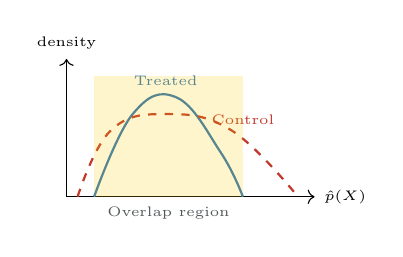
\begin{tikzpicture}[scale=0.7]
        % axis
        \draw[->] (0,0) -- (4.5,0) node[right,font=\tiny]{$\hat{p}(X)$};
        \draw[->] (0,0) -- (0,2.5) node[above,font=\tiny]{density};
        % treated dist
        \draw[accent, thick] plot[smooth,tension=0.7] coordinates {(0.5,0)(1.2,1.5)(2,1.8)(2.8,0.8)(3.2,0)};
        \node[accent, font=\tiny] at (1.8,2.1) {Treated};
        % control dist
        \draw[accent2, thick, dashed] plot[smooth,tension=0.7] coordinates {(0.2,0)(0.8,1.2)(1.8,1.5)(3,1.2)(4.2,0)};
        \node[accent2, font=\tiny] at (3.2,1.4) {Control};
        % overlap zone
        \fill[fill=eugold, fill opacity=0.2] (0.5,0) rectangle (3.2,2.2);
        \node[font=\tiny, color=asher] at (1.85,-0.3) {Overlap region};
      \end{tikzpicture}
      \end{center}
      \small Treated and control should overlap. Trim $\hat{p} < 0.05$ or $\hat{p} > 0.95$.
    \end{column}
  \end{columns}
\end{frame}

% ------------------------------------------------------------

\begin{frame}{Inverse Probability Weighting (IPW)}

  \textbf{Idea:} re-weight observations so that controls ``look like'' the treated group in terms of $X$.

  \medskip
  \textbf{IPW estimator for ATT:}
  \[
    \widehat{\tau}^{\text{ATT}}_{\text{IPW}} =
      \frac{1}{N_1} \sum_{i=1}^N \left[
        \frac{D_i \cdot Y_i}{1} -
        \frac{(1-D_i) \cdot \hat{p}(X_i)}{1-\hat{p}(X_i)} \cdot Y_i
      \right]
  \]

  Equivalently: run \texttt{reg Y i.D [aw=w]} with weights
  $w_i = D_i + (1-D_i)\dfrac{\hat{p}(X_i)}{1-\hat{p}(X_i)}$.

  \bigskip
  \begin{columns}[T]
    \begin{column}{0.48\textwidth}
      \begin{exampleblock}{Intuition}
        Control units with $\hat{p}$ close to 1 (``almost treated'') are up-weighted. Control units with $\hat{p}$ close to 0 (``nothing like treated'') are down-weighted.
      \end{exampleblock}
    \end{column}
    \begin{column}{0.48\textwidth}
      \begin{alertblock}{Warning: overlap matters}
        If $\hat{p}(X_i) \approx 1$ for some controls, weights explode. Always \textbf{trim} on propensity score before IPW ($0.1 < \hat{p} < 0.9$ as a starting rule).
      \end{alertblock}
    \end{column}
  \end{columns}
\end{frame}

% ------------------------------------------------------------

\begin{frame}{Doubly robust estimation}

  \textbf{Idea:} combine an \emph{outcome model} and a \emph{propensity score model}. Consistent if \emph{either} is correctly specified.

  \[
    \widehat{\tau}^{\text{DR}} =
      \frac{1}{N}\sum_i \left[
        \underbrace{\hat{\mu}_1(X_i) - \hat{\mu}_0(X_i)}_{\text{outcome model}}
        + \frac{D_i\bigl(Y_i - \hat{\mu}_1(X_i)\bigr)}{\hat{p}(X_i)}
        - \frac{(1-D_i)\bigl(Y_i - \hat{\mu}_0(X_i)\bigr)}{1-\hat{p}(X_i)}
      \right]
  \]

  where $\hat{\mu}_d(X) = E[Y|D=d, X]$ is the fitted outcome under treatment $d$.

  \pause
  \begin{block}{Insurance policy interpretation}
    If the outcome model is right $\Rightarrow$ the IPW correction term averages to zero $\Rightarrow$ DR is consistent.\\
    If the PS model is right $\Rightarrow$ the outcome model residuals are well-weighted $\Rightarrow$ DR is still consistent.\\
    You don't need both to be right --- but you should try hard on both.
  \end{block}

  \medskip
  \textbf{Stata:} \texttt{teffects ra} (outcome regression) \quad \texttt{teffects aipw} (doubly robust)
\end{frame}

% ============================================================
\section{Lab: Titanic and LaLonde}
% ============================================================

\begin{frame}{Lab overview}

  \begin{columns}[T]
    \begin{column}{0.48\textwidth}
      \begin{block}{Exercise 1 — Titanic (20 min)}
        \textbf{Question:} did first-class passengers have higher survival probability?\\[4pt]
        \textbf{Problem:} first-class passengers differ from others in age, sex --- confounders that also affect survival.\\[4pt]
        \textbf{Method:} subclassification on (sex $\times$ age group), compute ATE, ATT, ATU with explicit weights.\\[4pt]
        \textbf{Dataset:} \texttt{titanic.dta} (Mixtape)
      \end{block}
    \end{column}
    \begin{column}{0.48\textwidth}
      \begin{block}{Exercise 2 — LaLonde (70 min)}
        \textbf{Question:} did the NSW job-training programme raise earnings?\\[4pt]
        \textbf{Benchmark:} experimental ATT $\approx \$1{,}794$ (Lalonde 1986)\\[4pt]
        \textbf{Methods:} naive OLS $\rightarrow$ IPW $\rightarrow$ PS matching $\rightarrow$ CEM $\rightarrow$ doubly robust\\[4pt]
        \textbf{Datasets:} \texttt{nsw\_mixtape.dta} (experimental) + \texttt{cps\_mixtape.dta} (observational controls)
      \end{block}
    \end{column}
  \end{columns}

  \bigskip
  \centering
  \textbf{Script:} \texttt{Lab/L1\_matching.do}
\end{frame}

% ============================================================
% References
% ============================================================

\begin{frame}[allowframebreaks]{References}
  \bibliography{../Bibliography_base}
\end{frame}

\end{document}
